\chapter{Hardware}

\par En este capítulo se analiza el componente electrónico o de hardware, de aquí en más, estación de recolección de datos. Se aborda la elección de los elementos que lo componen, el diseño de interconexión, y la descripción del software que se ejecuta dentro del mismo. Detallándose, en esta última, las funcionalidades de obtención y persistencia de datos necesarios para el funcionamiento.

\section{Tecnologías evaluadas}
\label{SeccionTecnoEvalHardware}
    \par Para el funcionamiento del prototipo propuesto es necesario obtener datos digitales provenientes de múltiples sensores\footnote{Dispositivo capaz de recibir información de una magnitud del exterior y transformarla en otra magnitud, normalmente eléctrica, apta para ser cuantificada y manipulada} (temperatura y pH de líquidos;  temperatura y humedad ambiental); disponer de capacidad de almacenamiento para la persistencia de datos; e incorporar conectividad para transmisión de datos. De forma adicional, el componente debe poseer un tamaño reducido, de manera de no estorbar en las actividades de producción.

    \par Existen diferentes plataformas dentro de las cuales puede ser desarrollado un componente que cumpla los requerimientos antes mencionados. Raspberry\textsuperscript{\textregistered} y Arduino\textsuperscript{\textregistered} se destacan como las más utilizadas y con mayor comunidad, por tanto, luego se describen y comparan en detalle.
    
    \par Respecto de la recolección de datos, los sensores se describen abordando aspectos como costo económico, precisión y fiabilidad de los datos.
    
    \subsection{Análisis de elementos}
    \par A continuación se presenta el análisis de los elementos considerados para integrar la estación de recolección de datos.
    
        \subsubsection{Arduino: Microcontrolador}
        
            \par Arduino\textsuperscript{\textregistered} es una compañía de cultura libre\footnote{Corriente de pensamiento que promueve la libertad en la distribución y modificación de trabajos creativos basándose en el principio del contenido libre para distribuir o modificar trabajos y obras creativas.} que manufactura placas de desarrollo de hardware para construir dispositivos digitales e interactivos que pueden sensar y controlar objetos del mundo real. El software de Arduino\textsuperscript{\textregistered} consiste de dos elementos, un entorno de desarrollo (IDE) y un \textit{bootloader}\footnote{El bootloader de Arduino es un software alojado en la memoria flash que permite programar Arduino a través del puerto serie sin necesidad de usar un programador externo.} que es ejecutado de forma automática dentro del microcontrolador cuando este se enciende. Las placas Arduino se programan mediante un computador, usando comunicación serial. Generalmente el hardware (Figura \ref{boardArduino}) consiste de un microcontrolador\footnote{Un microcontrolador es un circuito integrado o chip que incluye en su interior las tres unidades funcionales de un ordenador: CPU, memoria y unidades de E/S.} Atmel AVR, conectado sobre una placa de circuito impreso con al menos 16 GPIO (\textit{General Purpose Input Output}) para entrada y salida de datos. A la misma se le pueden conectar placas de expansión (shields) que complementan la funcionalidad del modelo de placa empleada, agregando circuitería, sensores y módulos de comunicación externos a la placa original.
        
            \begin{figure}[h]
                \centering
                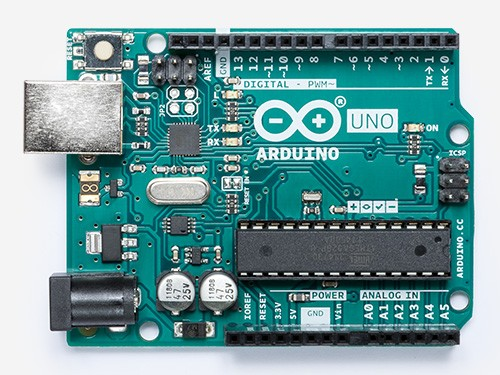
\includegraphics[scale=0.6]{hardware/Arduino.jpg}
                \caption{Placa Arduino\textsuperscript{\textregistered} UNO}
                \label{boardArduino}
            \end{figure}
        
        \subsubsection{Raspberry: Computadora de placa reducida}
            \par Raspberry\textsuperscript{\textregistered} Pi es un computador de placa reducida de bajo costo (SBC\footnote{Single Board Computer o SBC, es una computadora completa en un sólo circuito.}). Es decir, su diseño se centra en un sólo microprocesador con la RAM, E/S y todas las demás características de un computador funcional en una sola tarjeta que suele ser de tamaño reducido, y que tiene todo lo que necesita en la placa base. Estas placas son desarrolladas en Reino Unido por la Fundación Raspberry\textsuperscript{\textregistered} Pi. El software de las placas es open source, siendo su sistema operativo oficial una versión adaptada de Debian\footnote{Debian es un sistema operativo y una distribución de Software Libre, \url{www.debian.org}}, denominada Raspbian. También, es posible usar otros sistemas operativos como Windows 10. El hardware (Firgura \ref{boardRaspberry}), en todas sus versiones, incluye un procesador Broadcom, una memoria RAM, una GPU, puertos USB, HDMI, Ethernet y 40 pines GPIO. Ninguna de sus ediciones incluye memoria de almacenamiento pero si cuentan con un slot para memoria MicroSD. De forma adicional, es posible agregar placas de expansión HAT (Hardware Attached on Top) para agregar otras funcionalidades.
            
            \begin{minipage}{0.95\textwidth}
            
            \begin{center}
                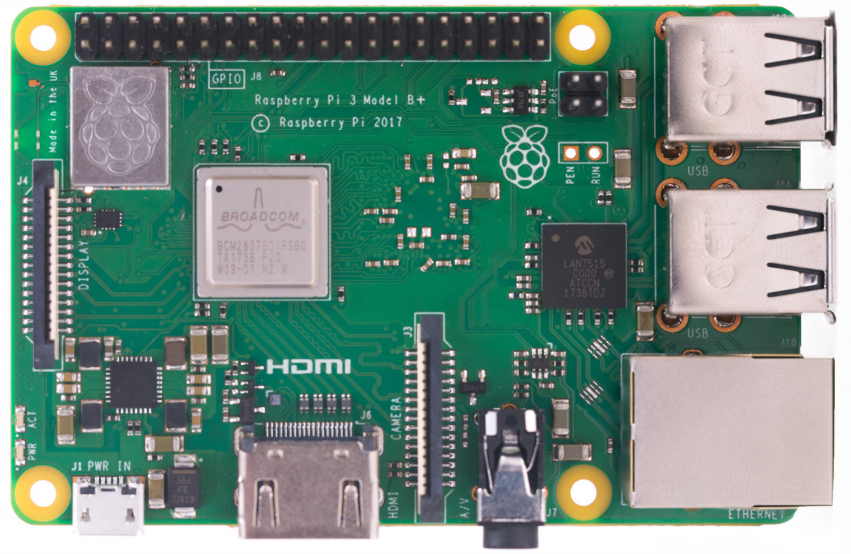
\includegraphics[scale=0.30]{hardware/raspberrypib3.jpg}
                
                \captionof{figure}{Placa Raspberry\textsuperscript{\textregistered} pi 3 B+}
                \label{boardRaspberry}
            \end{center}
            \end{minipage}
            \begin{minipage}{0.95\textwidth}
            \subsubsection{Comparación}
                \par En la Tabla \ref{CompHard}, se puede observar la comparación entre las dos placas descritas en la sección anterior. Los criterios de comparación utilizados se enfocaron en los requerimientos que este proyecto posee sobre dichos componentes.
            \end{minipage}
        
            
            \begin{center}
            \begin{tabularx}{\textwidth}{| X | X | X |}
            \hline
            \multicolumn{3}{|c|}{\textbf{Comparación de plataformas de hardware}} \\
            \hline
            Criterio de Comparación & Arduino\textsuperscript{\textregistered} & Raspberry\textsuperscript{\textregistered} pi \\
            \hline
            \hline
        
            Precio & \$440 (USD 17,00) & \$1900 (USD 61,00)
            \\ \hline
            Manejo de sensores & Digitales y analógicos & Digitales y analógicos
            \\ \hline
            Capacidad de procesamiento, memoria y almacenamiento & Procesador de 8 bits a 16Mhz, memoria de 2KB, sin almacenamiento (sin slot de expansión). & Procesador de 64 bits a 1.4Ghz, memoria de 1GB, sin almacenamiento (Slot memoria SD).
            \\ \hline
            Conectividad & Conexión USB (tipo B) x 1. Pueden adicionarse Shields Ethernet, Bluetooth o WiFi. & Conexión USB (tipo A) x 4, Ethernet 100M, WiFi 802.11n/ac, Bluetooth.
            \\ \hline
            Tamaño & 7.6 x 1.9 x 6.4 cm. & 8.6cm x 5.4cm x 1.7cm.
            \\ \hline

            
            \end{tabularx}
            \label{CompHard}
            %\captionof{table}{Comparación entre Arduino y Raspberry Pi}
            \end{center}
            
            \begin{center}
            \begin{tabularx}{\textwidth}{| X | X | X |}
                \hline
                \multicolumn{3}{|c|}{\textbf{Comparación de plataformas de hardware Cont.}} \\
                \hline
                Criterio de Comparación & Arduino\textsuperscript{\textregistered} & Raspberry\textsuperscript{\textregistered} pi \\
                \hline
                \hline
                
                Lenguaje de programación & Lenguaje Bajo Nivel. Gran comunidad y soporte. Se requiere de un computador para el desarrollo. & Lenguaje Alto Nivel. Gran comunidad y soporte. Se desarrolla directamente en el dispositivo.
                \\ \hline
                
                Persistencia de datos ante pérdida de alimentación eléctrica & Ninguna & Al utilizar una memoria SD, se obtiene persistencia de datos.
            \\ \hline
            \end{tabularx}
            \label{CompHardCont}
            \captionof{table}{Comparación entre Arduino y Raspberry Pi}
            \end{center}
            
        
    \subsection{Elementos utilizados}
    \label{subseccionElementosutilizados}
        \par A continuación se detallan los componentes de hardware utilizados.
        
        \subsubsection{Placa electrónica}
            \par En base al análisis de la Tabla \ref{CompHard}, la tecnología utilizada en este proyecto es \textbf{Raspberry\textsuperscript{\textregistered} Pi} (modelo Raspberry\textsuperscript{\textregistered} Pi 3 B+) debido a su mayor capacidad de procesamiento, almacenamiento, persistencia de datos y por poseer un lenguaje de programación de más alto nivel. Al incorporar, esta placa, conectividad inalámbrica de fábrica, posee la ventaja sobre Arduino\textsuperscript{\textregistered} de no requerir la instalación de placas externas para realizar este fin, siendo este tipo de conexiones necesarias para el desarrollo de este proyecto. Respecto al tamaño y precio, no presentan diferencias significativas de modo de influir en la elección propuesta.

        \subsubsection{Sensores}
            \par Tanto Arduino\textsuperscript{\textregistered} como Raspberry\textsuperscript{\textregistered} Pi pueden trabajar con sensores analógicos y digitales, debiendo en el caso del Raspberry\textsuperscript{\textregistered} utilizar un ADC\footnote{\textit{Analog Digital Converter}, Conversor Analogico Digital} para trabajar con sensores analógicos. Para cada tipo de sensor, existen numerosas opciones que se diferencian en cuanto a la precisión de las medidas, dónde esta característica aumenta en forma proporcional a su precio. 
            
            \par Para este proyecto se propone el desarrollo de un prototipo con un presupuesto limitado. Por tanto, no fue aplicado un criterio comparativo como el utilizado para las placas electrónicas, sino que, se buscaron sensores cuya relación precio/calidad sea adecuada y accesible al presupuesto de los alumnos proyectistas, enfocando esta decisión en la obtención de datos fiables para cumplir los objetivos del proyecto, y no en la precisión de los valores a obtener.
            
            \paragraph{Sensores de temperatura sumergibles:}Sensor que permite obtener valores de temperatura de un líquido a partir de su inmersión en él. Como fue mencionado antes, se decidió optar por un sensor que satisfaga la limitación precio/calidad y, de ser posible, que no requiera la utilización de un ADC con el fin de reducir costos y complejidad. Por esto, fue elegido el sensor digital DS18B20 (Figura \ref{SensorTemp}), cuyas características se describen a continuación:
            
                \begin{itemize}
                    \item Modelo: Sensor Digital Temperatura DS18B20 Cable Sumergible
                    \item Fabricante: Maxim
                    \item Microcontrolador: ATmega328P/
                    \item Voltaje de funcionamiento: 3,3V / 5V
                    \item Comunicación: Digital. Posee tres pines: VDD, Data, GND.
                    \item Precisión: 9 bits, tomando valores de -55°C - 125°C, con un margen de error de 0,5°C
                    \item Conexión: Cada sensor incorpora de fábrica un número de serie de 64 bits que permite conectar múltiples sensores en paralelo usando sólo una patilla como bus de datos
                \end{itemize}
                
                \begin{figure} [h]
                    \centering
                    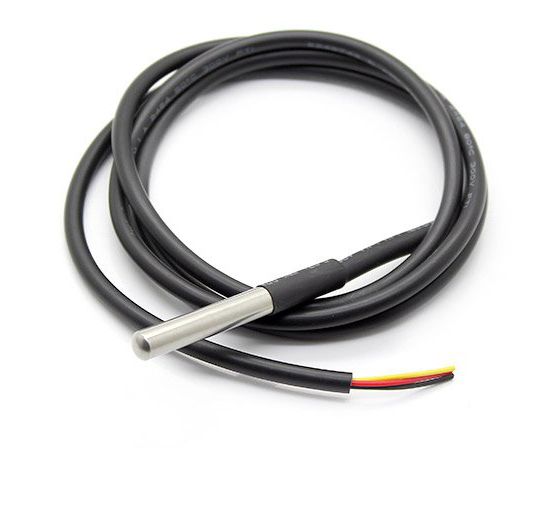
\includegraphics[scale=0.35]{hardware/ds18b20.jpg}
                    \caption{Sensor sumergible de temperatura - DS18B20}
                    \label{SensorTemp}
                \end{figure}
                
            \paragraph{Sensor de pH de líquidos:}Sensor electroquímico de pH\footnote{ Medida de acidez o alcalinidad de una disolución}, compuesto por un electrodo sumergible y una placa electrónica denominada sonda de pH (pH probe), que permiten transducir la actividad química del ion de hidrógeno en una señal eléctrica. (Figuras \ref{BoardPh} y \ref{phElectrode})
                
                \par A continuación se describen las características del sensor adquirido en base al presupuesto del proyecto:
                
                \begin{itemize}
                    \item Modelo: phMeter
                    \item Voltaje de funcionamiento : 5V
                    \item Comunicación: Analógica, cuenta con 6 pines. Conector tipo BNC
                    \item Precisión: ± 0.1pH, tomando valores de 0-14 pH
                    \item Temperatura de trabajo: 0ºC - 60ºC
                    \item Tiempo de Respuesta: 1 minuto
                \end{itemize}
                
                \begin{minipage}{0.95\textwidth}
                    \begin{center}
                    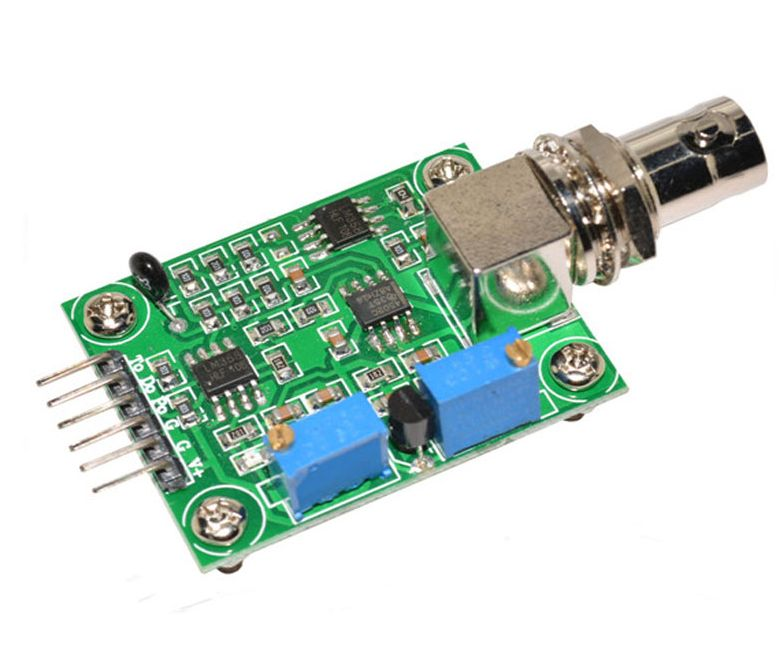
\includegraphics[scale=0.25]{hardware/phmoduloplaca.jpg}
                    \captionof{figure}{Placa sonda de pH}
                    \label{BoardPh}
                    \end{center}
                \end{minipage}
                
                \begin{minipage}{0.95\textwidth}
                    \begin{center}
                    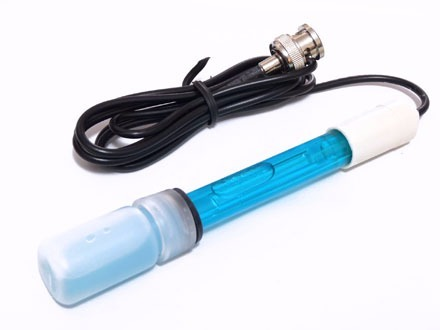
\includegraphics[scale=0.35]{hardware/electrododepH.jpg}
                    \captionof{figure}{Electrodo de pH}
                    \label{phElectrode}
                    \end{center}
                \end{minipage}
                
            \paragraph{Sensor de temperatura y humedad ambiental:}Sensor digital que permite realizar mediciones ambientales de temperatura y humedad relativa. Dados los condicionamientos antes planteados, el funcionamiento digital y las buenas prestaciones, se eligió el modelo de bajo costo DHT11 (Figura \ref{SensorDHT11}), sus características son descritas a continuación:
                \begin{itemize}
                    \item Modelo: DHT11
                    \item Fabricante: Adafruit
                    \item Voltaje de funcionamiento: 3V - 5V DC
                    \item Comunicación: Digital. Posee cuatro pines: VDD, Data, Idle, GND.
                    \item Rango de medición de temperatura: 0ºC a 50°C
                    \item Precisión de medición de temperatura: ±2.0 °C
                    \item Resolución Temperatura: 0.1°C
                    \item Rango de medición de humedad: 20\% a 90\% RH
                    \item Precisión de medición de humedad: 4\% RH
                    \item Resolución Humedad: 1\% RH
                    \item Tiempo de sensado: 2 seg
                \end{itemize}
                
                \begin{figure} [h]
                    \centering
                    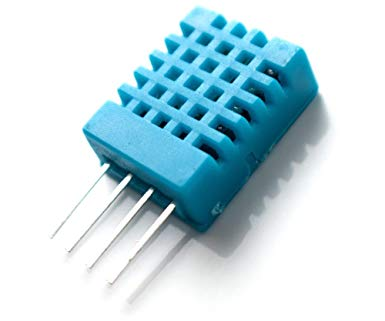
\includegraphics[scale=0.35]{hardware/dht11_.jpg}
                    \caption{Sensor de temperatura y humedad ambiente DHT11}
                    \label{SensorDHT11}
                \end{figure}

        
\section{Diseño}
    \par En las siguientes secciones se analiza y define la estrategia utilizada para abordar el desarrollo del componente de Hardware.
    
    \subsection{Lista de elementos}
    \label{subsectionListaElemHard}
    Con base en lo descrito en la sección \ref{SeccionTecnoEvalHardware} se lista, finalmente, la siguiente serie de elementos para el diseño del componente.
        \begin{itemize}
            \item 6 sensores digitales de temperatura sumergibles DS18B20 con 2 metros de extensión por cable
            \item 1 sensor digital de temperatura y humedad ambiente Adafruit DHT11
            \item 1 sensor de pH analógico ( Electrodo y Plaqueta controladora)
            \item 1 Conversor Analógico / Digital (Arduino\textsuperscript{\textregistered} Uno)
            \item 1 Raspberry\textsuperscript{\textregistered} Pi 3 B+
            \item Resistencias electrónicas (4.7 k$\Omega$, 10 k$\Omega$)
            \item Protoboard con cables
            \item Fuente de alimentación microUSB 5v 2.1A
            \item Memoria Micro SD Clase 10 16GB
        \end{itemize}
        
    \subsection{Consideraciones previas}
        \par En este apartado se describen restricciones inherentes al funcionamiento del sistema que debieron ser consideradas para el diseño del mismo. Cada una se detalla justificando la decisión de diseño que se optó.
        
        \paragraph{Medición de pH:} 
            La obtención de este valor se realiza mediante el sensor electroquímico antes mencionado en la sección \ref{SeccionTecnoEvalHardware}. Por cuestiones inherentes al funcionamiento, este sensor, requiere de al menos 2 minutos para estabilizar el resultado obtenido (medición).
            
            \par Respecto de la variación de las mediciones de pH con la temperatura, (M. E. Mohammd Ali y O. A. Razag Sharif, 2015) expresa que la medición es afectada de dos maneras. Por un lado, al valor de pH de la solución, cuya corrección directa no puede ser realizada, dado que cada muestra de pH tiene una relación\footnote{Coeficiente de temperatura de la solución  $ = \Delta pH/ ^{\circ}C $} entre pH y temperatura única. Sin embargo, una compensación de pH debe ser realizada a través de una calibración utilizando soluciones \textit{buffers} de pH estándares. Por otro lado, al efecto de la temperatura sobre la sensibilidad del electrodo de pH, el cual puede ser corregido y cuya desviación depende de cada electrodo. El fabricante del electrodo utilizado en este desarrollo provee la Tabla \ref{tablePhvsTemp} de desvíos. 
            
            \begin{figure}[h] 
                \centering
                %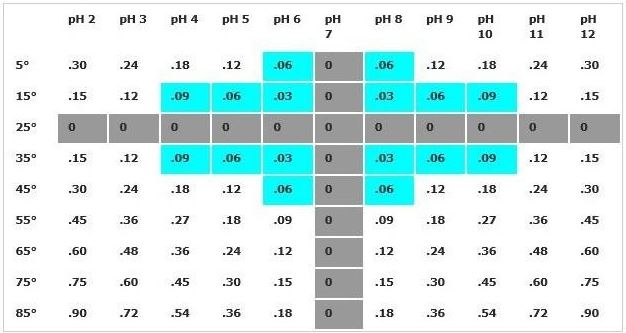
\includegraphics[scale=0.9]{errorMedicionPh.jpg}
                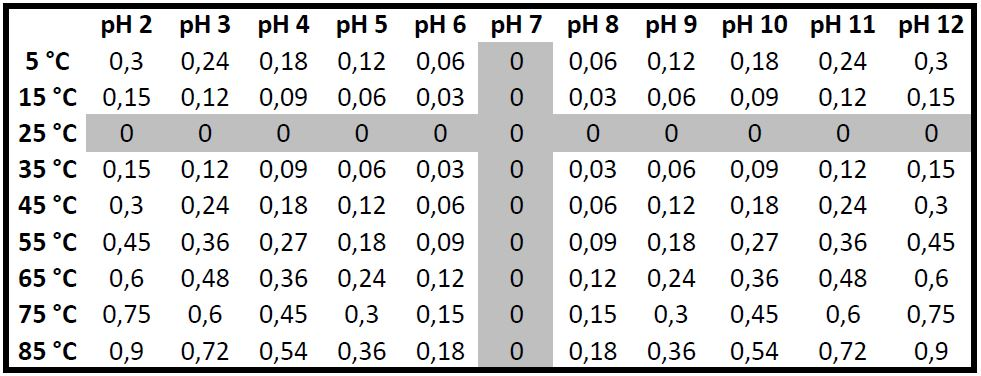
\includegraphics[scale=0.6]{hardware/ErrorMedicionPH.jpg}
                \caption{Error de medición de pH respecto a la temperatura de la solución}
                \label{tablePhvsTemp}
            \end{figure}
            
            \par Por las características mencionadas, el intervalo de medición  de pH, para este proyecto, es de 2 minutos (El usuario puede aumentar este intervalo si lo requiere) asumiendo así el correspondiente error. El desvío de medición del pH ocasionado por la temperatura de sensado es ajustado por un sensor sumergible de temperatura destinado a este propósito, junto a la Tabla \ref{tablePhvsTemp}.
        
        \paragraph{Medición de temperatura:} 
            Debido a que el objeto involucrado en la medición es un líquido, se opta por un sensor de temperatura sumergible.
    
        \paragraph{Almacenamiento:} 
        Cada experimento almacenado requiere aproximadamente de 1 MB de memoria. De esta manera, al utilizarse la memoria descrita en \ref{subsectionListaElemHard}, una vez ocupado los 8 GB necesarios para el sistema operativo y las herramientas quedan disponibles aproximadamente 8 GB para almacenamiento de experimentos. A razón de 1 MB por experimento, da un aproximado de 8.192 experimentos almacenadas sin alcanzar el límite de almacenamiento. 
        
        \paragraph{Desconexión de sensores:} 
             Ante la posible desconexión de los sensores, el sistema debe ser capaz de identificar la falla. Luego, reportar el error para considerar el desperfecto para próximos experimentos y evitar incorporar el valor erróneo a las estadísticas de funcionamiento. Dado que se plantea al sistema como una herramienta de asistencia al productor, se opta por no cancelar el experimento bajo esta situación debido a los costos de la materia prima involucrada.
            
            
    \subsection{Diseño del componente}
            \par Durante el inicio de la etapa de diseño de la estación de recolección de datos se decidió dividir las tareas en dos módulos: Subcapa de software y subcapa de hardware.
            
            \subsubsection{Subcapa de software}
                \par El sistema operativo utilizado para el Raspberry\textsuperscript{\textregistered} es \textit{Raspbian}\footnote{\url{https://www.raspberrypi.org/downloads/raspbian/}}, una distribución basada en Debian Linux provista por el fabricante de la placa.
                
               \par El desarrollo de las funcionalidades de software se realiza en Python. Esta opción se elige como primer alternativa al contar con una amplia comunidad de desarrolladores, librerías y es recomendado por el sitio oficial de Raspberry\textsuperscript{\textregistered} (Raspberry\textsuperscript{\textregistered} Official Page, 2018) para la programación con GPIO.
                
                \par Para la gestión de los datos, se emplea el motor de base de datos MySQL. Se justifica esta elección por su simpleza de uso, mínimos requerimientos para un correcto funcionamiento y la existencia de herramientas de interacción con \textit{Scripts} en lenguaje Python.
                
                \par Respecto del funcionamiento del componente, una serie de funciones (\textit{Scripts}) escritas en lenguaje Python realizan las tareas de recolección de datos e inserción en la base de datos. Estas funciones son ejecutadas mediante comandos \textit{bash}\footnote{https://www.debian.org/doc/manuals/debian-reference/ch01.es.html} del sistema al que a las que se les adjuntan los parámetros necesarios para el proceso de obtención de datos.
                \par Estas funciones se repetirán durante los diferentes ciclos de muestreo definidos acorde a la duración del experimento y la frecuencia de medición. Ejecutando en cada iteración las funciones necesarias para los fines requeridos:
                    
                    \begin{itemize}
                        \item Obtención de datos de sensores: Cada sensor utiliza una función específica desarrollada de forma particular para garantizar su correcto funcionamiento. De esta manera, se abordan de manera eficaz los posibles inconvenientes (\textit{bugs}) que puedan ser identificados.
                        
                        \item Insertar datos en la Base de Datos: Los datos obtenidos en cada secuencia de medición se insertan en la base de datos a partir de un identificador (Id) proporcionado como parámetro de la función.
                    \end{itemize}
                
                \paragraph{Diagrama de Base de Datos:} La Figura \ref{fig:DiagramaBdRasp} ubicada en el Anexo, presenta el diagrama de base de datos utilizado. El mismo, consiste de tres tablas relacionadas mediante claves foráneas (\textit{foreign keys}): \textit{Maceración}, \textit{Experimento} y \textit{SensedValues}. 
                
                
            \subsubsection{Subcapa de hardware} 
                \par En la Figura \ref{fig:EsquemaHardware} del Anexo, se presenta un esquema simplificado de conexiones de la subcapa de Hardware. En dicho esquema se encuentran identificadas las entradas (sensores y conversor) y la salida (API REST) del Raspberry\textsuperscript{\textregistered} Pi.
                
                \par Como se mencionó en \ref{subseccionElementosutilizados}, para poder procesar la señal analógica del sensor de pH es necesario que previamente ésta sea digitalizada. Para tal función se emplea un Arduino\textsuperscript{\textregistered} Uno en modo esclavo para utilizar su DAC interno de 10 bits.
        
    
\section{Implementación del diseño}
    \par A continuación son descriptas mediante diagramas las implementaciones de las subcapas utilizadas.
    %%% Corroborar la oración de acá arriba
    \subsection{Subcapa de software}
        \par En el diagrama de flujo de la Figura \ref{FlujoPython} se muestra el flujo de funcionamiento que cumple las funcionalidades que se desprenden del diseño.

        \begin{figure}
        \centering
            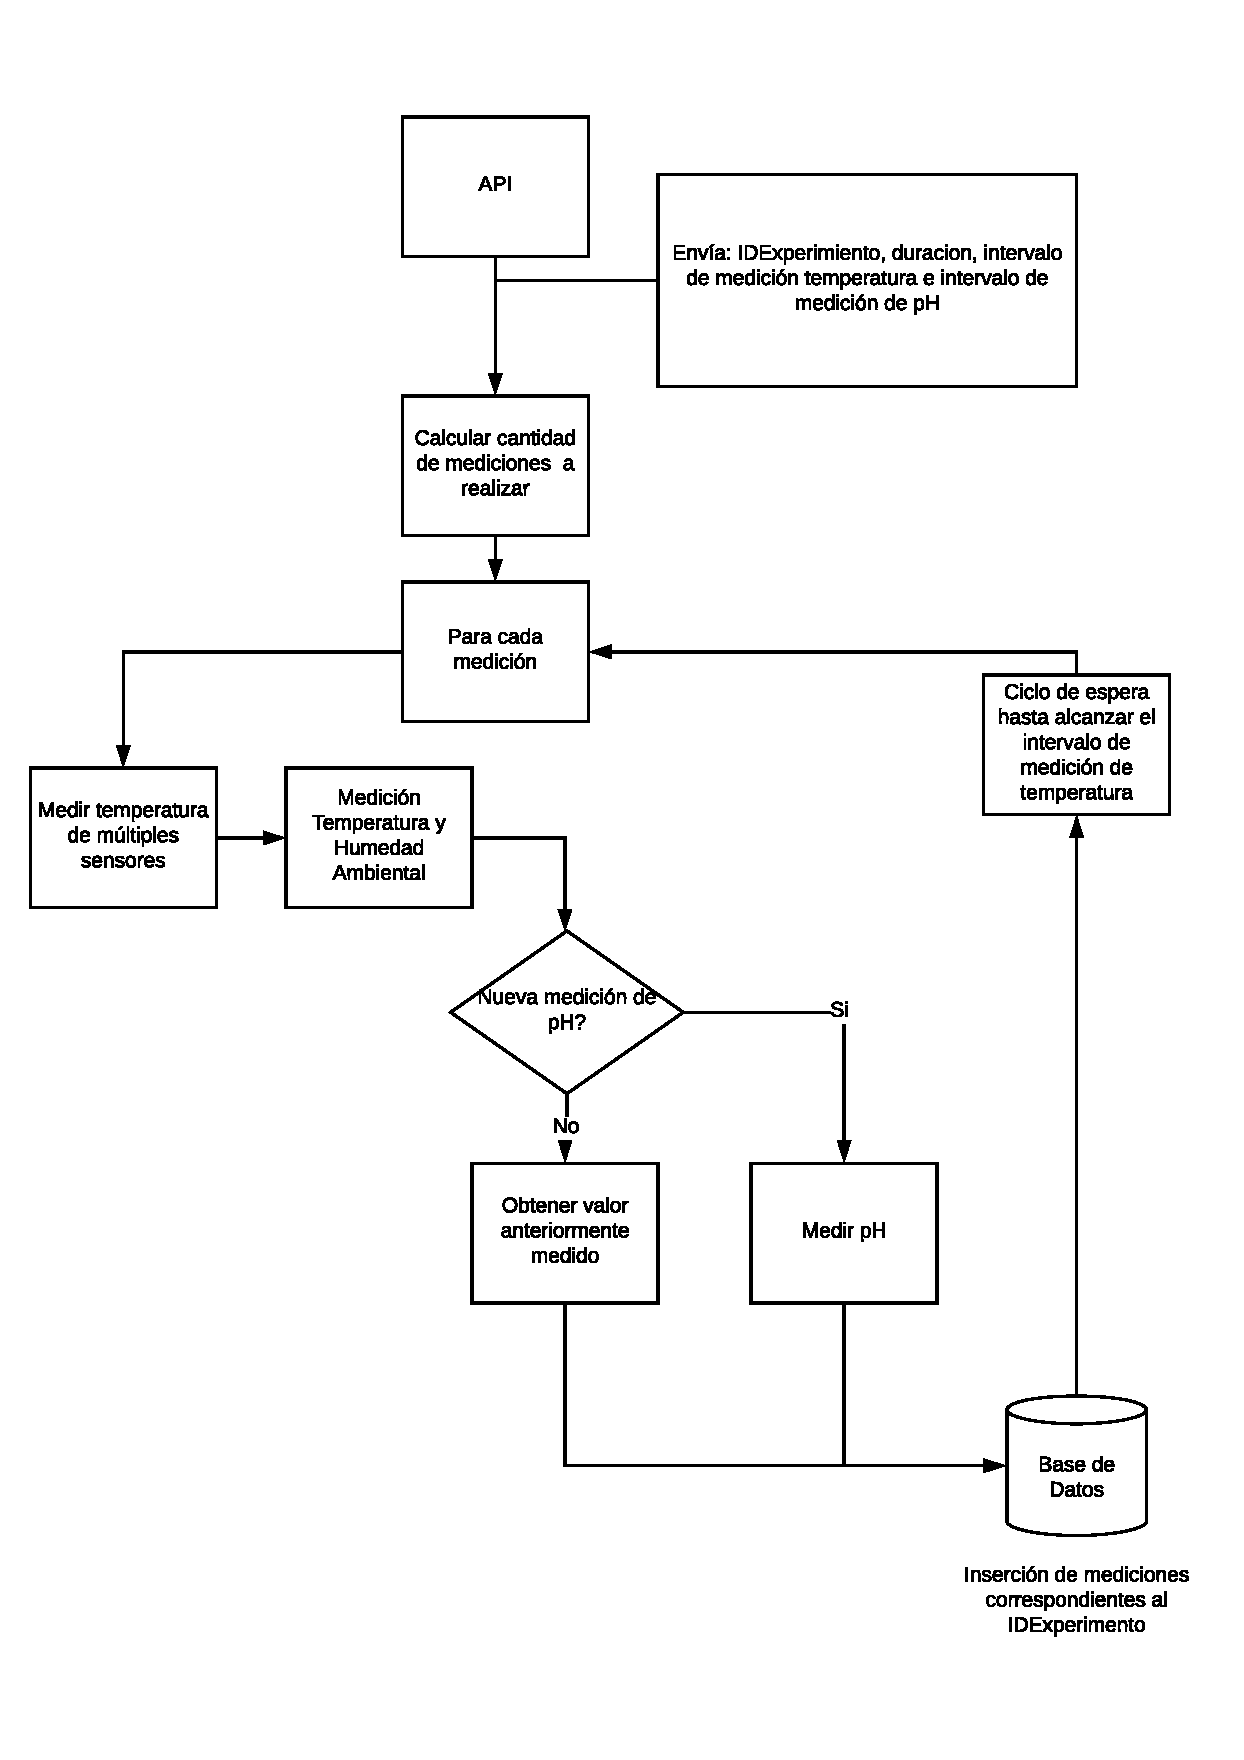
\includegraphics[scale=0.75]{hardware/DiagramadeFlujoPython.pdf}
            \caption{Diagrama de flujo del funcionamiento del software }
            \label{FlujoPython}
        \end{figure}

    \subsection{Subcapa de hardware}
        \par En las siguientes subsecciones se muestran los diagramas de conexión de cada sensor con la placa Raspberry, siguiendo el diseño general de la la Figura \ref{fig:EsquemaHardware} del Anexo.

    \subsubsection{Conexión del sensor de pH}
        \par En la Figura \ref{fig:ConexionSensorpH} se muestra el diagrama de conexión del sensor de pH, conformado por el sensor electroquímico, electrodo y "sonda de pH". Este último, se encuentra conectado a una placa Arduino\textsuperscript{\textregistered} UNO que realiza la función de conversor Analógico-Digital enviando los datos analógicos obtenidos por el sensor como una señal digital al Raspberry\textsuperscript{\textregistered} mediante conexión Serial USB.
        
        \begin{figure}[h]
            \centering
            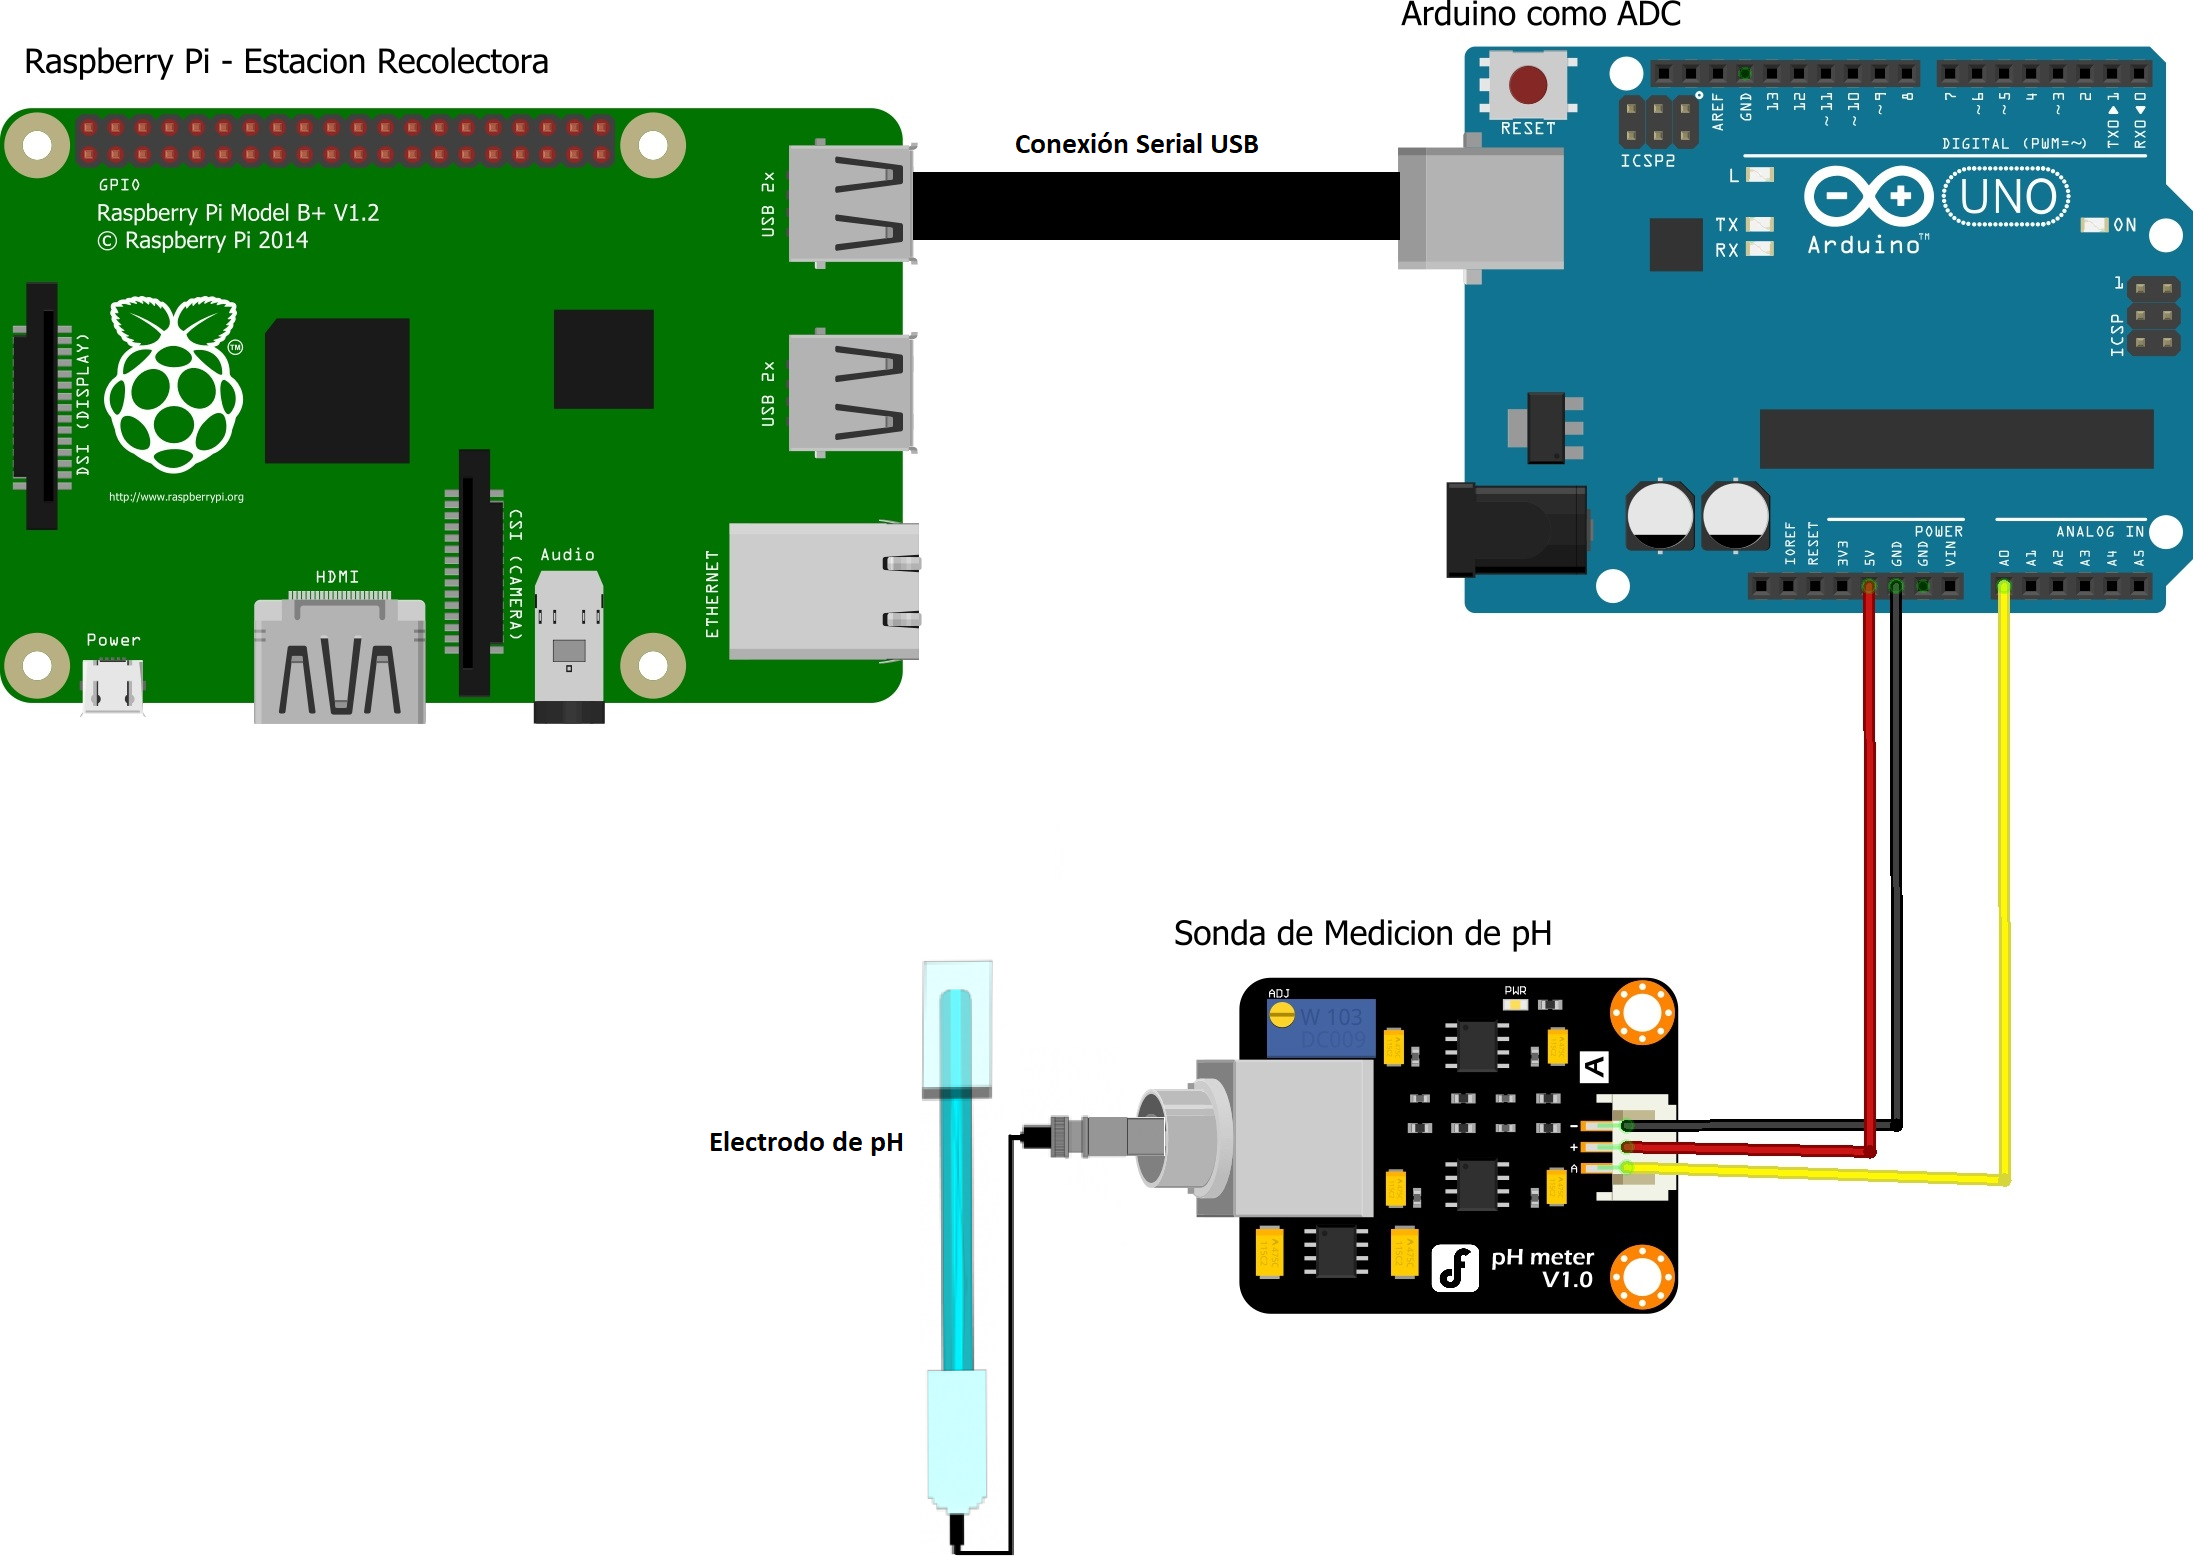
\includegraphics[scale=0.25]{hardware/DiagramaSensordepH_bb2.jpg}
            \caption{Diagrama de conexión del sensor de pH}
            \label{fig:ConexionSensorpH}
        \end{figure}

    \subsubsection{Conexión del sensor de temperatura sumergible}

        \par Para poder realizar las mediciones del líquido se utiliza un sensor de temperatura sumergible (véase \ref{subseccionElementosutilizados}). Dicho sensor requiere la conexión de un resistencia de $4.7k\Omega$ entre el pin de datos (Data) y el de corriente continua (VDD). En forma adicional, este sensor incorpora la posibilidad de conexión de múltiples sensores en serie mediante el bus I2C\footnote{Bus desarrollado por Philips\textsuperscript{\textregistered} para envío de datos en serie entre un circuito maestro y uno o varios esclavos}. Bajo esta dinámica, cada sensor DS18B20 dispone de un código de identificación único que le permite ser identificado de forma unívoca por la placa Raspberry\textsuperscript{\textregistered}. En la figura \ref{fig:ConexionTemperatura} se presenta el diagrama de conexión de estos sensores.
        %\begin{minipage}{0.95 \textwidth}
        \begin{figure}[h]
            \centering
            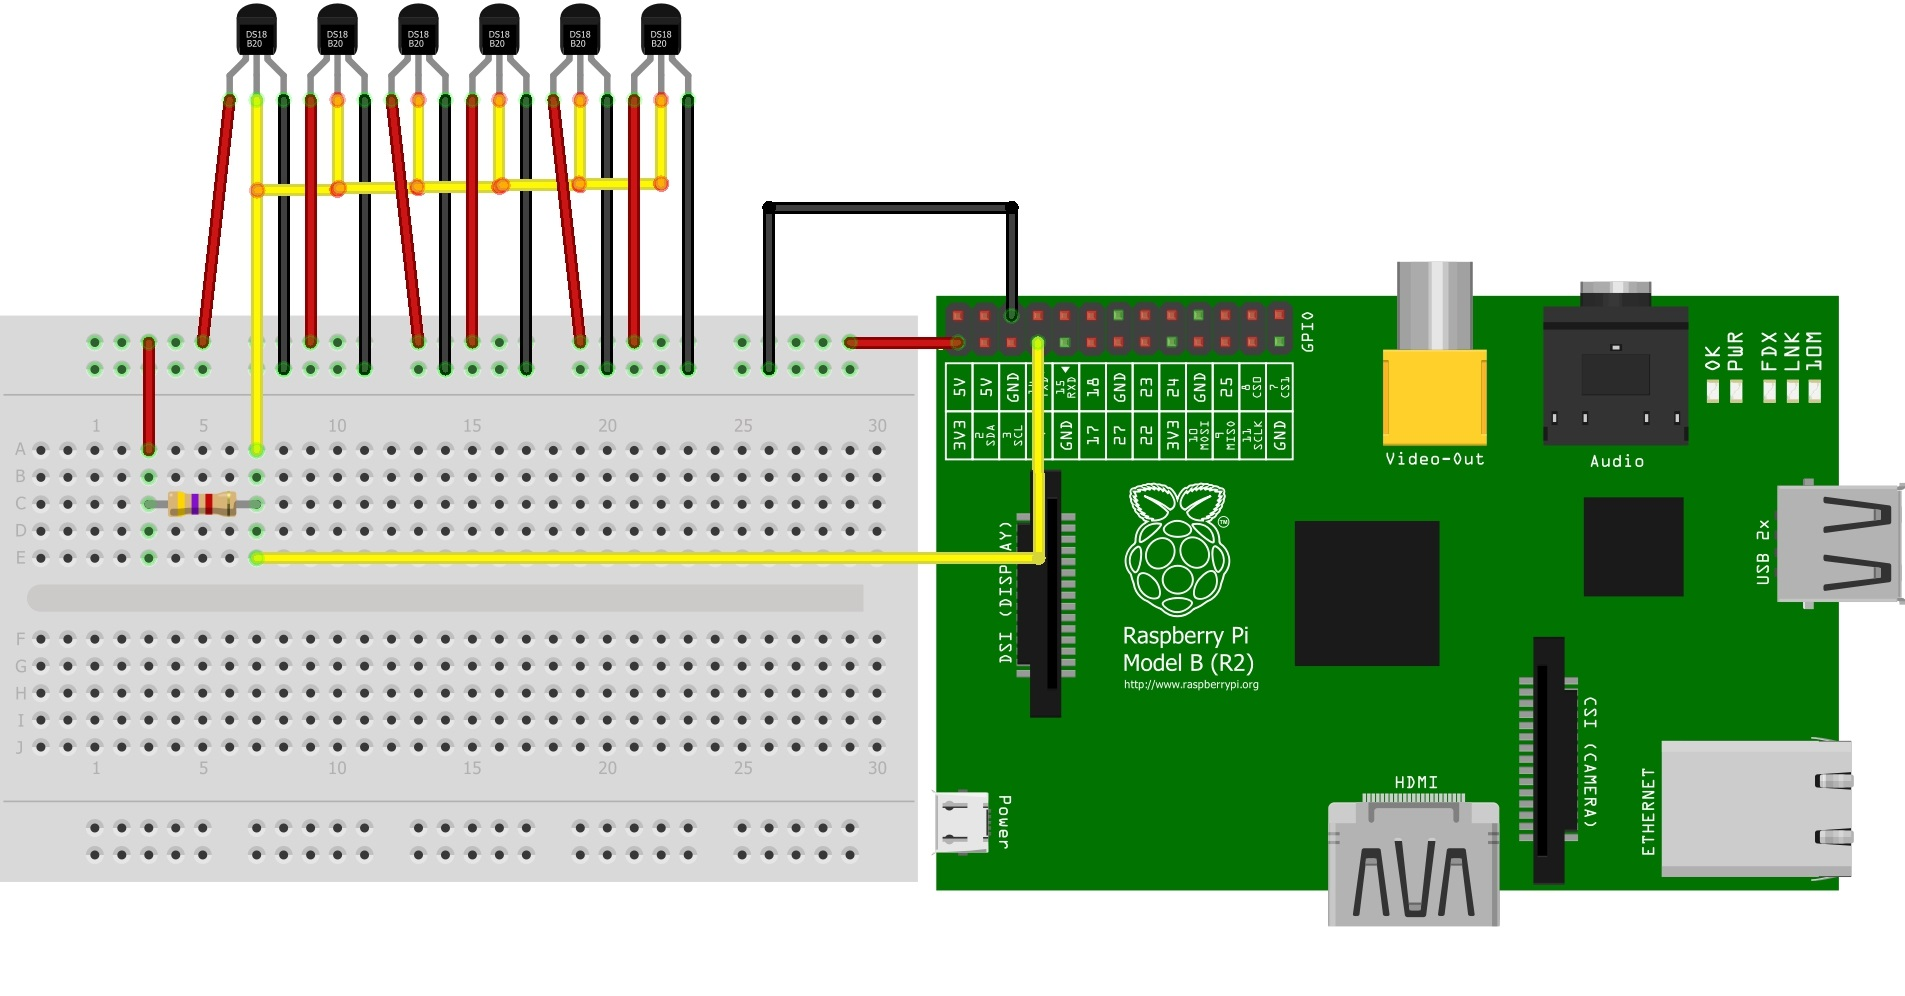
\includegraphics[scale = 0.8]{DiagramaSensordeTemp_bb.jpg}
            \caption{Diagrama de conexión de los sensores de temperatura}
            \label{fig:ConexionTemperatura}
        \end{figure}
        
    \subsubsection{Conexión del sensor temperatura y humedad ambiental}
        \par Para recolectar los valores de temperatura y humedad ambiental se utiliza un sensor dedicado (véase \ref{subseccionElementosutilizados}). Este sensor, al igual que el anterior, requiere la conexión de los pines de corriente continua (VDD) y el de datos (Data) mediante una resistencia de $4.7k\Omega$. En la figura \ref{fig:EsquemaDHT11} se muestra el esquema de conexión.
    %\begin{minipage}{0.95 \textwidth}    
        \begin{figure}[h]
            \centering
            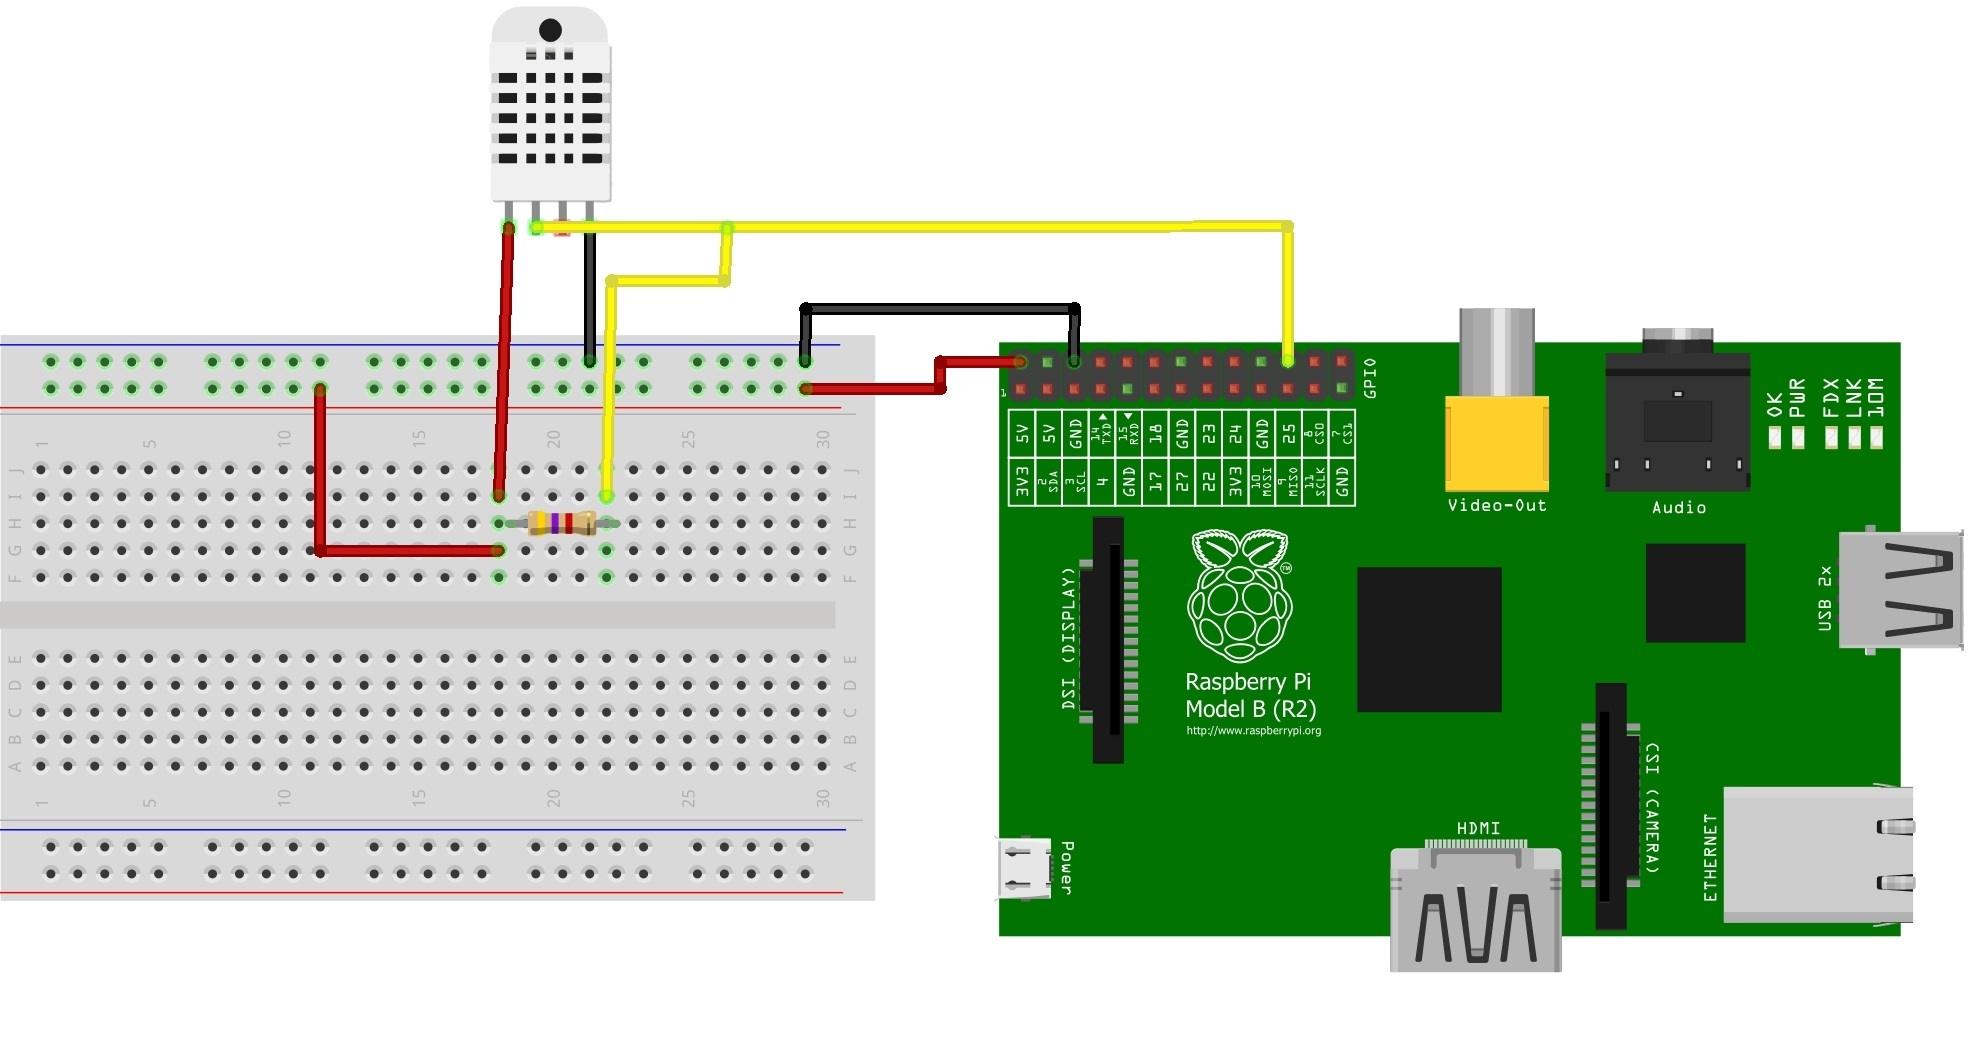
\includegraphics[scale = 0.8]{DiagramaSensorDHT11_bb.jpg}
            \caption{Diagrama de conexión del sensor DHT11}
            \label{fig:EsquemaDHT11}
        \end{figure}

\section{Ensamble completo}

    \par Finalmente, en la Figura \ref{fig:EsquemaCompletoHardware} se exhibe mediante una imagen fotográfica la integración de todos los componentes, en conjunto, la estación de recolección de datos.\\
%\end{minipage}
%\begin{minipage}{0.95 \textwidth}

    \begin{figure}[t]
    \centering
        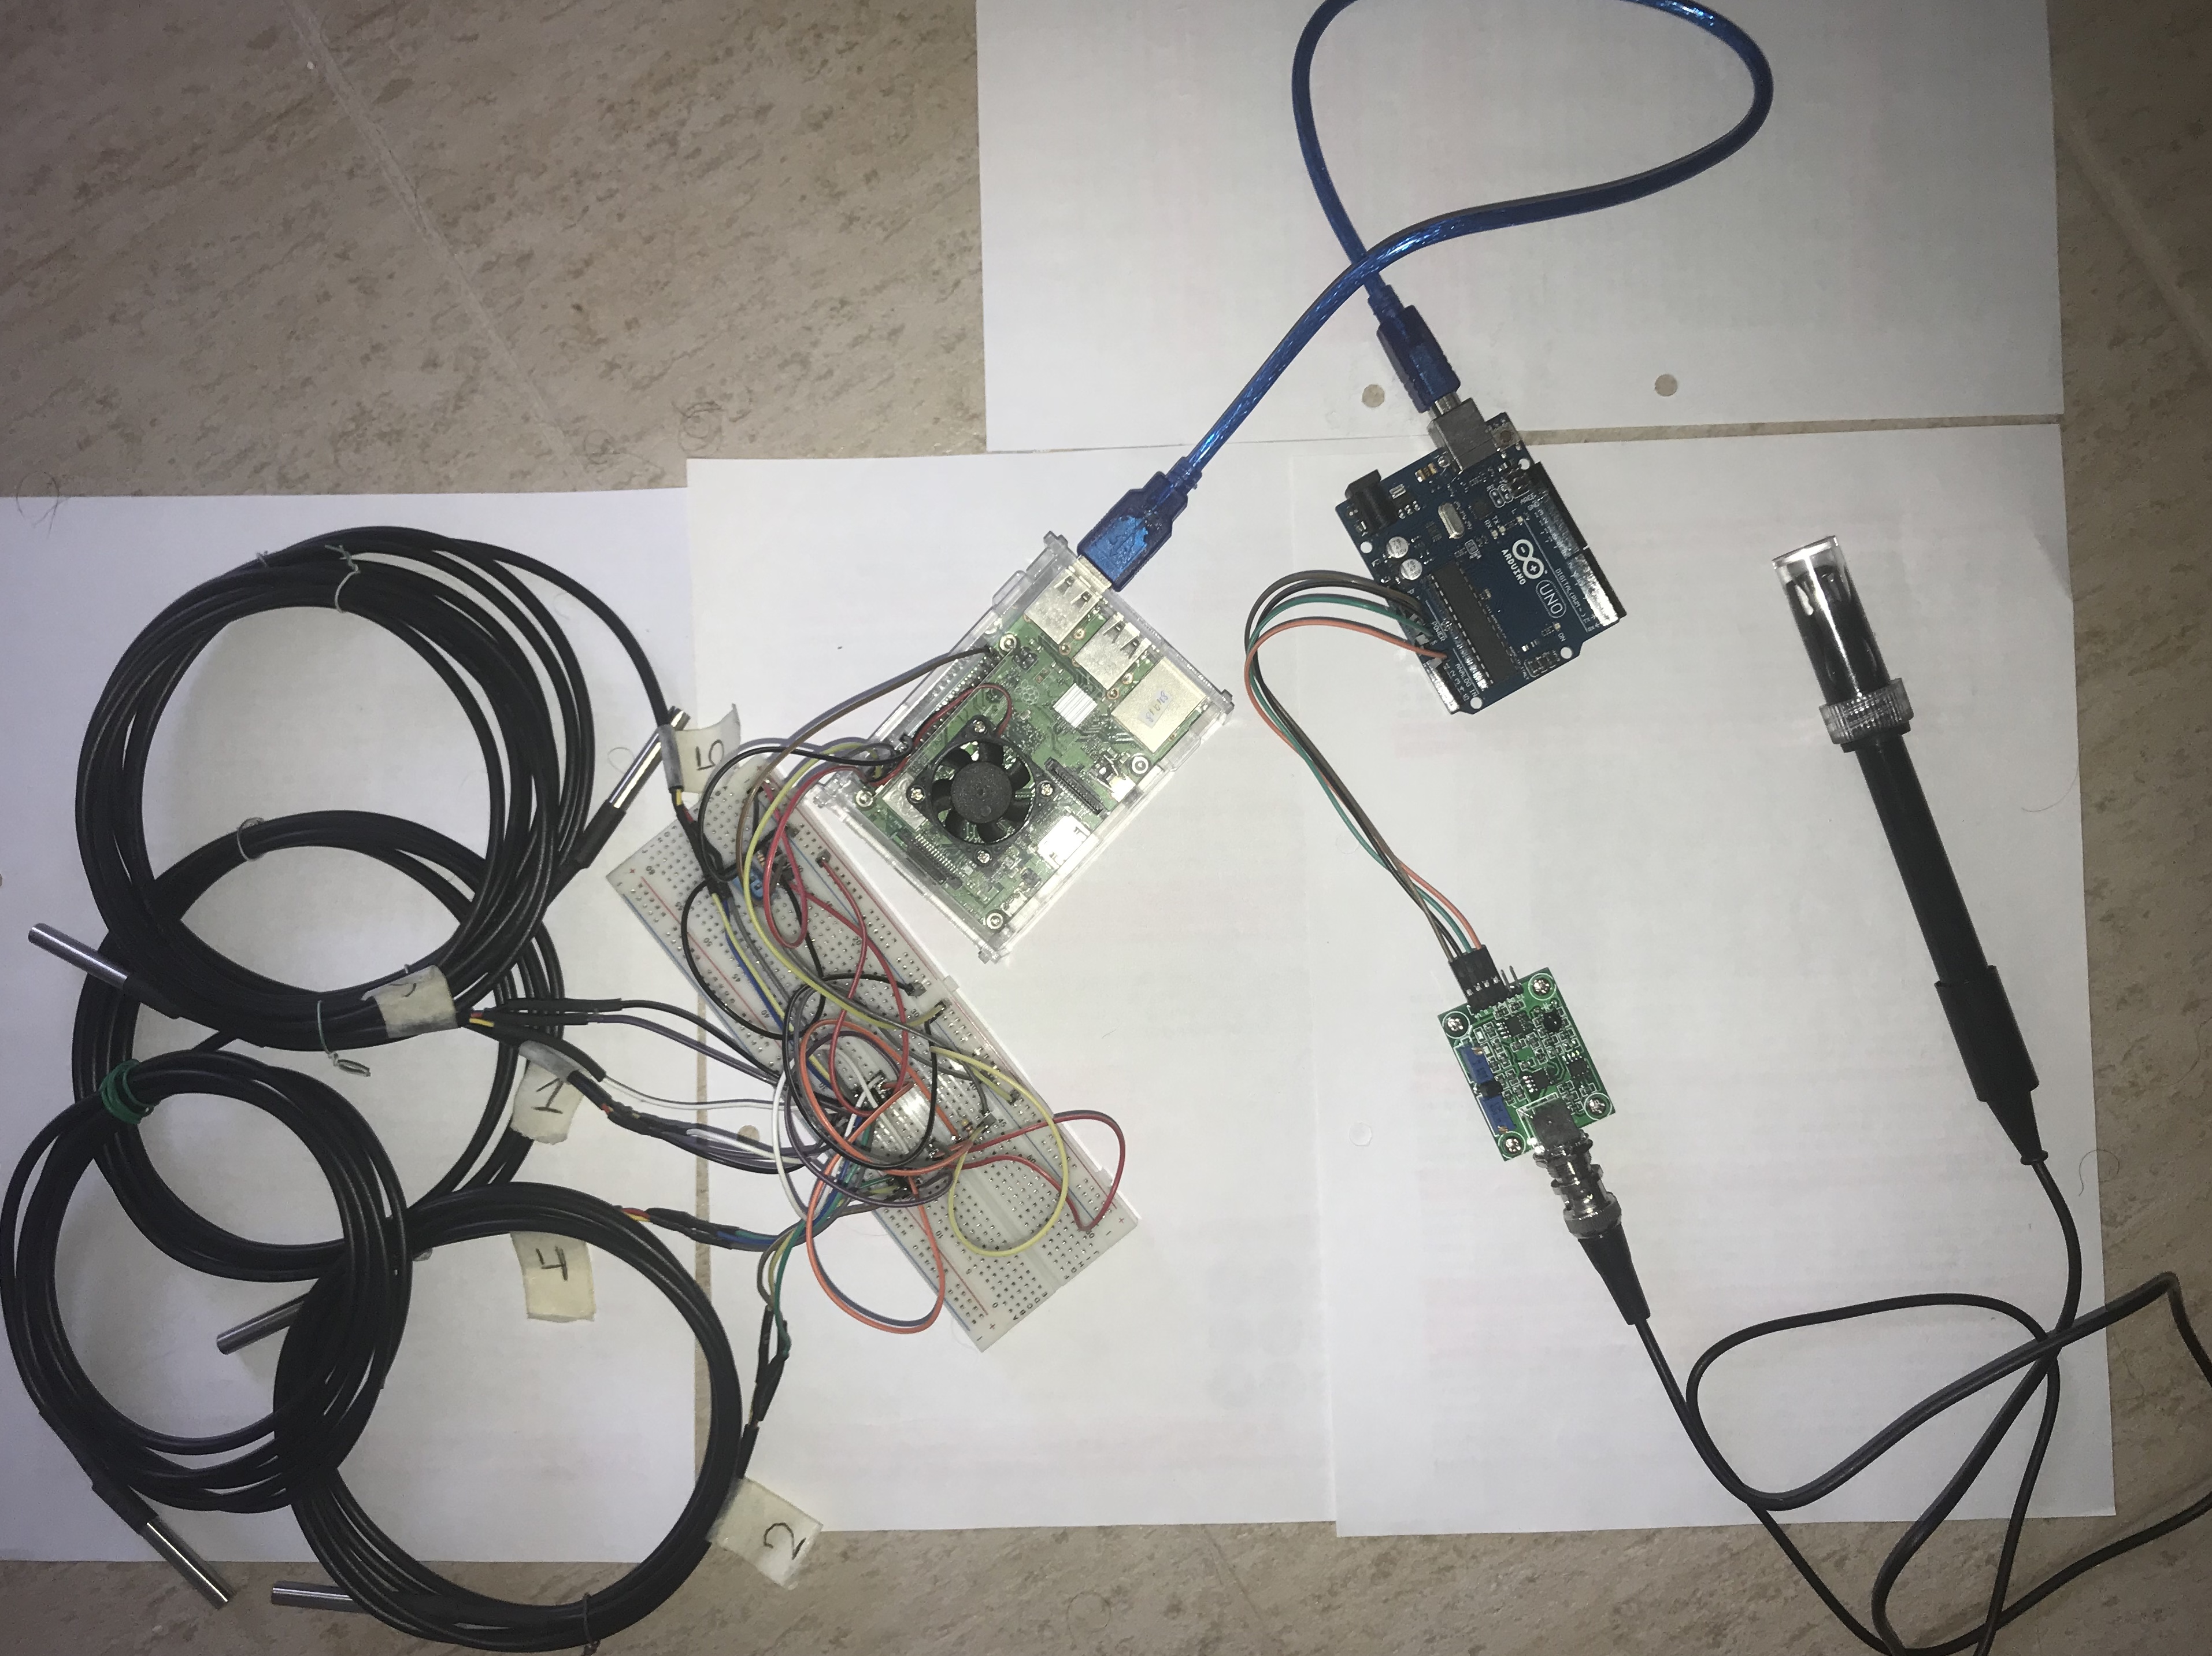
\includegraphics[scale=0.11]{hardware/SistemaEnsamblado.jpeg}
        \captionof{figure}{Fotografía de la estación de recolección de datos}
        \label{fig:EsquemaCompletoHardware}
    \end{figure}

    
%\end{minipage}